% Options for packages loaded elsewhere
\PassOptionsToPackage{unicode}{hyperref}
\PassOptionsToPackage{hyphens}{url}
\PassOptionsToPackage{dvipsnames,svgnames,x11names}{xcolor}
%
\documentclass[
  letterpaper,
  DIV=11,
  numbers=noendperiod]{scrartcl}

\usepackage{amsmath,amssymb}
\usepackage{lmodern}
\usepackage{iftex}
\ifPDFTeX
  \usepackage[T1]{fontenc}
  \usepackage[utf8]{inputenc}
  \usepackage{textcomp} % provide euro and other symbols
\else % if luatex or xetex
  \usepackage{unicode-math}
  \defaultfontfeatures{Scale=MatchLowercase}
  \defaultfontfeatures[\rmfamily]{Ligatures=TeX,Scale=1}
\fi
% Use upquote if available, for straight quotes in verbatim environments
\IfFileExists{upquote.sty}{\usepackage{upquote}}{}
\IfFileExists{microtype.sty}{% use microtype if available
  \usepackage[]{microtype}
  \UseMicrotypeSet[protrusion]{basicmath} % disable protrusion for tt fonts
}{}
\makeatletter
\@ifundefined{KOMAClassName}{% if non-KOMA class
  \IfFileExists{parskip.sty}{%
    \usepackage{parskip}
  }{% else
    \setlength{\parindent}{0pt}
    \setlength{\parskip}{6pt plus 2pt minus 1pt}}
}{% if KOMA class
  \KOMAoptions{parskip=half}}
\makeatother
\usepackage{xcolor}
\setlength{\emergencystretch}{3em} % prevent overfull lines
\setcounter{secnumdepth}{-\maxdimen} % remove section numbering
% Make \paragraph and \subparagraph free-standing
\ifx\paragraph\undefined\else
  \let\oldparagraph\paragraph
  \renewcommand{\paragraph}[1]{\oldparagraph{#1}\mbox{}}
\fi
\ifx\subparagraph\undefined\else
  \let\oldsubparagraph\subparagraph
  \renewcommand{\subparagraph}[1]{\oldsubparagraph{#1}\mbox{}}
\fi

\usepackage{color}
\usepackage{fancyvrb}
\newcommand{\VerbBar}{|}
\newcommand{\VERB}{\Verb[commandchars=\\\{\}]}
\DefineVerbatimEnvironment{Highlighting}{Verbatim}{commandchars=\\\{\}}
% Add ',fontsize=\small' for more characters per line
\usepackage{framed}
\definecolor{shadecolor}{RGB}{241,243,245}
\newenvironment{Shaded}{\begin{snugshade}}{\end{snugshade}}
\newcommand{\AlertTok}[1]{\textcolor[rgb]{0.68,0.00,0.00}{#1}}
\newcommand{\AnnotationTok}[1]{\textcolor[rgb]{0.37,0.37,0.37}{#1}}
\newcommand{\AttributeTok}[1]{\textcolor[rgb]{0.40,0.45,0.13}{#1}}
\newcommand{\BaseNTok}[1]{\textcolor[rgb]{0.68,0.00,0.00}{#1}}
\newcommand{\BuiltInTok}[1]{\textcolor[rgb]{0.00,0.23,0.31}{#1}}
\newcommand{\CharTok}[1]{\textcolor[rgb]{0.13,0.47,0.30}{#1}}
\newcommand{\CommentTok}[1]{\textcolor[rgb]{0.37,0.37,0.37}{#1}}
\newcommand{\CommentVarTok}[1]{\textcolor[rgb]{0.37,0.37,0.37}{\textit{#1}}}
\newcommand{\ConstantTok}[1]{\textcolor[rgb]{0.56,0.35,0.01}{#1}}
\newcommand{\ControlFlowTok}[1]{\textcolor[rgb]{0.00,0.23,0.31}{#1}}
\newcommand{\DataTypeTok}[1]{\textcolor[rgb]{0.68,0.00,0.00}{#1}}
\newcommand{\DecValTok}[1]{\textcolor[rgb]{0.68,0.00,0.00}{#1}}
\newcommand{\DocumentationTok}[1]{\textcolor[rgb]{0.37,0.37,0.37}{\textit{#1}}}
\newcommand{\ErrorTok}[1]{\textcolor[rgb]{0.68,0.00,0.00}{#1}}
\newcommand{\ExtensionTok}[1]{\textcolor[rgb]{0.00,0.23,0.31}{#1}}
\newcommand{\FloatTok}[1]{\textcolor[rgb]{0.68,0.00,0.00}{#1}}
\newcommand{\FunctionTok}[1]{\textcolor[rgb]{0.28,0.35,0.67}{#1}}
\newcommand{\ImportTok}[1]{\textcolor[rgb]{0.00,0.46,0.62}{#1}}
\newcommand{\InformationTok}[1]{\textcolor[rgb]{0.37,0.37,0.37}{#1}}
\newcommand{\KeywordTok}[1]{\textcolor[rgb]{0.00,0.23,0.31}{#1}}
\newcommand{\NormalTok}[1]{\textcolor[rgb]{0.00,0.23,0.31}{#1}}
\newcommand{\OperatorTok}[1]{\textcolor[rgb]{0.37,0.37,0.37}{#1}}
\newcommand{\OtherTok}[1]{\textcolor[rgb]{0.00,0.23,0.31}{#1}}
\newcommand{\PreprocessorTok}[1]{\textcolor[rgb]{0.68,0.00,0.00}{#1}}
\newcommand{\RegionMarkerTok}[1]{\textcolor[rgb]{0.00,0.23,0.31}{#1}}
\newcommand{\SpecialCharTok}[1]{\textcolor[rgb]{0.37,0.37,0.37}{#1}}
\newcommand{\SpecialStringTok}[1]{\textcolor[rgb]{0.13,0.47,0.30}{#1}}
\newcommand{\StringTok}[1]{\textcolor[rgb]{0.13,0.47,0.30}{#1}}
\newcommand{\VariableTok}[1]{\textcolor[rgb]{0.07,0.07,0.07}{#1}}
\newcommand{\VerbatimStringTok}[1]{\textcolor[rgb]{0.13,0.47,0.30}{#1}}
\newcommand{\WarningTok}[1]{\textcolor[rgb]{0.37,0.37,0.37}{\textit{#1}}}

\providecommand{\tightlist}{%
  \setlength{\itemsep}{0pt}\setlength{\parskip}{0pt}}\usepackage{longtable,booktabs,array}
\usepackage{calc} % for calculating minipage widths
% Correct order of tables after \paragraph or \subparagraph
\usepackage{etoolbox}
\makeatletter
\patchcmd\longtable{\par}{\if@noskipsec\mbox{}\fi\par}{}{}
\makeatother
% Allow footnotes in longtable head/foot
\IfFileExists{footnotehyper.sty}{\usepackage{footnotehyper}}{\usepackage{footnote}}
\makesavenoteenv{longtable}
\usepackage{graphicx}
\makeatletter
\def\maxwidth{\ifdim\Gin@nat@width>\linewidth\linewidth\else\Gin@nat@width\fi}
\def\maxheight{\ifdim\Gin@nat@height>\textheight\textheight\else\Gin@nat@height\fi}
\makeatother
% Scale images if necessary, so that they will not overflow the page
% margins by default, and it is still possible to overwrite the defaults
% using explicit options in \includegraphics[width, height, ...]{}
\setkeys{Gin}{width=\maxwidth,height=\maxheight,keepaspectratio}
% Set default figure placement to htbp
\makeatletter
\def\fps@figure{htbp}
\makeatother

\KOMAoption{captions}{tableheading}
\makeatletter
\makeatother
\makeatletter
\makeatother
\makeatletter
\@ifpackageloaded{caption}{}{\usepackage{caption}}
\AtBeginDocument{%
\ifdefined\contentsname
  \renewcommand*\contentsname{Table of contents}
\else
  \newcommand\contentsname{Table of contents}
\fi
\ifdefined\listfigurename
  \renewcommand*\listfigurename{List of Figures}
\else
  \newcommand\listfigurename{List of Figures}
\fi
\ifdefined\listtablename
  \renewcommand*\listtablename{List of Tables}
\else
  \newcommand\listtablename{List of Tables}
\fi
\ifdefined\figurename
  \renewcommand*\figurename{Figure}
\else
  \newcommand\figurename{Figure}
\fi
\ifdefined\tablename
  \renewcommand*\tablename{Table}
\else
  \newcommand\tablename{Table}
\fi
}
\@ifpackageloaded{float}{}{\usepackage{float}}
\floatstyle{ruled}
\@ifundefined{c@chapter}{\newfloat{codelisting}{h}{lop}}{\newfloat{codelisting}{h}{lop}[chapter]}
\floatname{codelisting}{Listing}
\newcommand*\listoflistings{\listof{codelisting}{List of Listings}}
\makeatother
\makeatletter
\@ifpackageloaded{caption}{}{\usepackage{caption}}
\@ifpackageloaded{subcaption}{}{\usepackage{subcaption}}
\makeatother
\makeatletter
\@ifpackageloaded{tcolorbox}{}{\usepackage[many]{tcolorbox}}
\makeatother
\makeatletter
\@ifundefined{shadecolor}{\definecolor{shadecolor}{rgb}{.97, .97, .97}}
\makeatother
\makeatletter
\makeatother
\ifLuaTeX
  \usepackage{selnolig}  % disable illegal ligatures
\fi
\IfFileExists{bookmark.sty}{\usepackage{bookmark}}{\usepackage{hyperref}}
\IfFileExists{xurl.sty}{\usepackage{xurl}}{} % add URL line breaks if available
\urlstyle{same} % disable monospaced font for URLs
\hypersetup{
  pdftitle={Empirical Research},
  pdfauthor={Adham Rishmawi},
  colorlinks=true,
  linkcolor={blue},
  filecolor={Maroon},
  citecolor={Blue},
  urlcolor={Blue},
  pdfcreator={LaTeX via pandoc}}

\title{Empirical Research}
\author{Adham Rishmawi}
\date{}

\begin{document}
\maketitle
\ifdefined\Shaded\renewenvironment{Shaded}{\begin{tcolorbox}[borderline west={3pt}{0pt}{shadecolor}, frame hidden, enhanced, breakable, boxrule=0pt, interior hidden, sharp corners]}{\end{tcolorbox}}\fi

\hypertarget{setting-up-packages-and-knitting-options}{%
\subsection{Setting up packages and knitting
options}\label{setting-up-packages-and-knitting-options}}

\hypertarget{loading-in-data-from-source}{%
\subsection{Loading in data from
source}\label{loading-in-data-from-source}}

\begin{Shaded}
\begin{Highlighting}[]
\NormalTok{data1 }\OtherTok{\textless{}{-}} \FunctionTok{read.csv}\NormalTok{(}\StringTok{"https://sldr.netlify.app/data/sustainable{-}livelihoods.csv"}\NormalTok{)}\SpecialCharTok{|\textgreater{}}
  \FunctionTok{drop\_na}\NormalTok{(Increased\_Yield) }\SpecialCharTok{|\textgreater{}}
  \FunctionTok{drop\_na}\NormalTok{(Increased\_Knowledge)}\SpecialCharTok{|\textgreater{}}
  \FunctionTok{drop\_na}\NormalTok{(Food\_Ran\_Out)}\SpecialCharTok{|\textgreater{}}
  \FunctionTok{arrange}\NormalTok{(Partner)}
\end{Highlighting}
\end{Shaded}

\begin{itemize}
\tightlist
\item
  We dropped the NA instances from the main predictors and response
  variable we would like to use!
\end{itemize}

\hypertarget{economic-question}{%
\subsection{Economic question}\label{economic-question}}

The economic question was derived out of the description of the data-set
I found:

Q. \textbf{do the programs affect the individual's intellectuality and
yield where it makes sure that there is less food deprivation occurring
more often. (is there a association between food\_ran\_out and
increased\_knowledge and increased\_yield?)}

\textbf{Data Description:}

World Renew implemented Sustainable Livelihoods, a five-year project in
Bangladesh, Honduras, Mali, Mozambique, and Tanzania to enhance
livelihood security for vulnerable households. The Sustainable
Livelihoods program worked to build the adaptive capacity of individual
households, as well as communities, to manage climate change risks.
Poverty in the communities where the program operated is manifested by
poor health, low incomes, food insecurity, landlessness, illiteracy and
underemployment. Small-scale farmers are challenged by declining soil
fertility, lack of secure land tenure, erratic weather and lack of
access to credit and inputs. These conditions lead to food shortages and
poor nutrition and health. In addition, poor urban households lack
skills for employment and financing for small enterprises.

About 80\% of the program participants were subsistence farmers who
depend on rain-fed agriculture for their livelihoods. The other 20\% of
program participants belonged to poor households in urban areas, many of
them living in slums where living conditions are crowded and unsanitary.

Participants had access to one or more training opportunities designed
to promote or improve financial savings, leadership, literacy, and
agricultural practices.

World Renew collected data to measure the impact of the Sustainable
Livelihoods program including variables:

\begin{itemize}
\item
  \texttt{Participant\_ID}, unique ID for each participant
\item
  \texttt{Country}
\item
  \texttt{Partner} organization
\item
  \texttt{Gender} of participant
\item
  \texttt{Town} where the person lives
\item
  \texttt{District} where the person lives
\item
  \texttt{Age\_Group} of the person completing the survey
\item
  \texttt{Savings\_Program}, whether the person participated in the
  financial savings program
\item
  \texttt{Leadership\_Program}, whether the person participated in the
  leadership training program
\item
  \texttt{Agriculture\_Program}, whether the person participated in the
  sustainable agriculture program
\item
  \texttt{Literacy\_Program}, whether the person participated in the
  literacy program
\item
  \texttt{n\_Programs}, number of programs the person participated in
\item
  \texttt{FFS}, food frequency score (a measure of food security)
\item
  \texttt{FDS}, food diversity score (a measure of food security and
  diverse diet)
\item
  \texttt{Months\_Enough\_Food}, months (out of the 12 in the past year)
  where the person had enough food
\item
  \texttt{Months\_Insufficient\_Food}, months (out of the 12 in the past
  year) where the person \emph{did not} have enough food
\item
  \texttt{Business\_Plan}, whether the person had a business plan
\item
  \texttt{Management\_Confidence}, whether the person had confidence in
  their management skills
\item
  \texttt{Sustainable\_Ag\_Practices}, whether the person practiced
  sustainable agriculture
\item
  \texttt{Minimum\_Tillage}, whether the person used minimum tillage (a
  sustainable farming practice)
\item
  \texttt{Soil\_Covered}, whether the person kept soil covered (a
  sustainable farming practice)
\item
  \texttt{Crop\_Rotation}, whether the person rotated crops (a
  sustainable farming practice)
\item
  \texttt{All\_Sustainable\_Practices}, whether the person did all three
  sustainable farming practices: minimum tillage, soil covered, and crop
  rotation
\item
  \texttt{Increased\_Yield}, whether the person had had increased
  farming yield after program participation
\item
  \texttt{Drought\_Disease\_Resistance}, whether the person was growing
  drought- or disease-resistant seeds
\item
  \texttt{Sustainable\_Useful}, whether the person thought sustainable
  farming practices were useful
\item
  \texttt{Literacy\_Helped}, whether the person thought the literacy
  program helped them
\item
  \texttt{Increased\_Knowledge}, whether the person said their knowledge
  had increased
\item
  \texttt{Food\_Ran\_Out}, whether or not the person ran out of food
  during the study period
\item
  \texttt{Vegetables}, whether the person, others in the family, or no
  one ate vegetables
\item
  \texttt{Fruits}, whether the person, others in the family, or no one
  ate fruits
\end{itemize}

\textbf{Data reference/other conducted studies:}

\begin{itemize}
\item
  Link to UN Sustainability development and Promoting Development
  Cooperation
  \href{www.un.org/en/ecosoc/docs/pdfs/fina_08-45773.pdf}{here.}
\item
  link to a statement about the USA contribution to this type of
  initiative
  \href{https://www.usaid.gov/news-information/press-releases/may-12-2022-usaid-launches-new-205-million-climate-change-and-environmental}{here.}

  \hypertarget{section}{%
  \subsection{}\label{section}}

  \hypertarget{is-economic-question-well-motivated}{%
  \subsection{Is Economic question well
  motivated?}\label{is-economic-question-well-motivated}}
\item
  This question has not been proposed yet directly and is worth asking
  because the initiative will indicate to the provider of this program a
  factor to see if it is worthwhile.
\item
  The links provided above have done studies that are quite different
  but this question will focus more on the intellectuality increase and
  if that decreases the amount of food deprivation in these countries.
\item
  Whether this question indicates to us true or not it will give us a
  right step into indicating the more precise question we should be
  asking.

  \hypertarget{predictor-choices-for-model}{%
  \subsection{Predictor choices for
  model}\label{predictor-choices-for-model}}
\item
  \texttt{Increased\_Knowledge} and \texttt{Increased\_Yield}

  \begin{itemize}
  \tightlist
  \item
    Justification: This i thought would be a great predictor to pair up
    with increase\_yield because they are both binary options which we
    can study instances where both are either 1 or zeros and see how
    they influence my response variable.
  \end{itemize}
\item
  \texttt{Age\_Group}

  \begin{itemize}
  \tightlist
  \item
    Justification: this an additional predictor that i thought would
    influence my response variable because certain ages might be a
    contributor to the reason why they ran out of food or the reason
    their knowledge changed differently so I included it.
  \end{itemize}
\item
  \texttt{Gender}

  \begin{itemize}
  \tightlist
  \item
    Justification: this was a included because I believe cultural
    aspects and circumstances would alter the rates at which people ran
    out of food and learned.
  \end{itemize}
\item
  \texttt{(1\textbar{}Partner)}

  \begin{itemize}
  \tightlist
  \item
    Justification: the Random effects I based it on The Partner because
    i believed it would be a bad traditional predictor because all the
    Organizations included have the same goal so theoretical it should
    be a bad predictor. It also fits the criteria we said in class that
    it must be a location, time, or identity which it is. I did not get
    any convergence problems so that's a good identification that it is
    a good RE effect.
  \end{itemize}
\item
  All other columns and variables:

  \begin{itemize}
  \tightlist
  \item
    Justification: I wanted to stay within the rule of thumb for this
    test and make sure that my predictors did not go beyond the
    threshold. Other predictors would have played into distorting the
    correlation between my response variable and predictors.
  \end{itemize}

  \hypertarget{response-variable-justification}{%
  \subsection{Response variable
  Justification}\label{response-variable-justification}}
\item
  the reason I choose \texttt{Food\_Ran\_Out} is because I want to do
  binary evaluation because this variable is either no or yes. I had
  other options such as \texttt{Months\_insufficient\_Food} but I
  thought this response variable would be more suitable because it is
  whether they completely ran out or not which is more simpler.

  \hypertarget{operationalization-of-each-of-the-variables}{%
  \subsection{Operationalization of each of the
  variables}\label{operationalization-of-each-of-the-variables}}
\item
  the degree of measurement for our response variable is whether the
  people ran out of food more frequently less when we saw an increase in
  knowledge from these programs.
\item
  we will also tie an interaction with \texttt{Increased\_Yield} and
  \texttt{Increased\_Knowledge} to see if we can observe a corresponding
  reaction from both. (indicating if we see an increase in knowledge
  that in turn, results in a increased crop yield)
\item
  The quality of this data is derived from a established source so it
  has trust-able factors which means the extractions from it are
  tangible.

  \hypertarget{motivation-to-justify-research-question}{%
  \subsection{Motivation to justify Research
  question}\label{motivation-to-justify-research-question}}
\end{itemize}

here are examples of researches that did similar studies under different
constraints:

\begin{itemize}
\item
  \textbf{The Impact of Livelihood Assets on the Food Security of
  Farmers in Southern Iran during the COVID-19 Pandemic.} The authors
  review a range of case studies and program evaluations from around the
  world to assess the impact of sustainable livelihoods programs on key
  indicators of food security, such as access to food, dietary
  diversity, and food utilization.
  \href{https://www.ncbi.nlm.nih.gov/pmc/articles/PMC8156269/}{Link}
\item
  \textbf{Enhancing Agricultural Productivity and Sustainability through
  Sustainable Livelihoods Programs: Evidence from Ghana.} This study by
  Mensah and colleagues examines the impact of a sustainable livelihoods
  program on agricultural productivity and sustainability in Ghana. The
  authors use a randomized controlled trial design to assess the
  effectiveness of the program in improving farmers' access to inputs,
  promoting sustainable farming practices, and increasing yields.
  \href{https://www.ncbi.nlm.nih.gov/pmc/articles/PMC6740034/}{Link}
\item
  \textbf{An Assessment of Poverty Alleviation Measures and Sustainable
  Livelihood Capability of Farm Households in Rural China: A Sustainable
  Livelihood Approach.} This study by Kumar and colleagues explores the
  relationship between sustainable livelihoods programs and knowledge
  acquisition in rural India. The authors use a mixed-methods approach
  to assess the impact of the program on farmers' knowledge of
  sustainable farming practices and their ability to adapt to climate
  change risks. \href{https://www.mdpi.com/2077-0472/11/12/1230}{Link}
\end{itemize}

\hypertarget{quantitative-research}{%
\subsection{Quantitative research}\label{quantitative-research}}

\hypertarget{initial-demonstrating-graphs}{%
\paragraph{Initial demonstrating
graphs}\label{initial-demonstrating-graphs}}

\begin{Shaded}
\begin{Highlighting}[]
\NormalTok{int\_graph1 }\OtherTok{\textless{}{-}} \FunctionTok{gf\_boxplot}\NormalTok{(Food\_Ran\_Out }\SpecialCharTok{\textasciitilde{}}\NormalTok{ Increased\_Knowledge }\SpecialCharTok{|}\NormalTok{ Increased\_Yield ,  }\AttributeTok{data =}\NormalTok{ data1) }\SpecialCharTok{\%\textgreater{}\%}
  \FunctionTok{gf\_jitter}\NormalTok{(}\AttributeTok{alpha =} \FloatTok{0.3}\NormalTok{, }\AttributeTok{width =} \FloatTok{0.2}\NormalTok{) }\SpecialCharTok{\%\textgreater{}\%}
   \FunctionTok{gf\_labs}\NormalTok{(}\AttributeTok{subtitle =} \StringTok{"Initial graph elaborating assiocation between knowledge and the decrease of no food"}\NormalTok{,}
          \AttributeTok{title =} \StringTok{"Assiocation Graph for interaction"}\NormalTok{,}
          \AttributeTok{x =} \StringTok{" Increase of Knowledge"}\NormalTok{,}
          \AttributeTok{y =} \StringTok{"Did they have food?"}\NormalTok{, }
\NormalTok{           )}

\NormalTok{int\_graph1}
\end{Highlighting}
\end{Shaded}

\begin{figure}[H]

{\centering 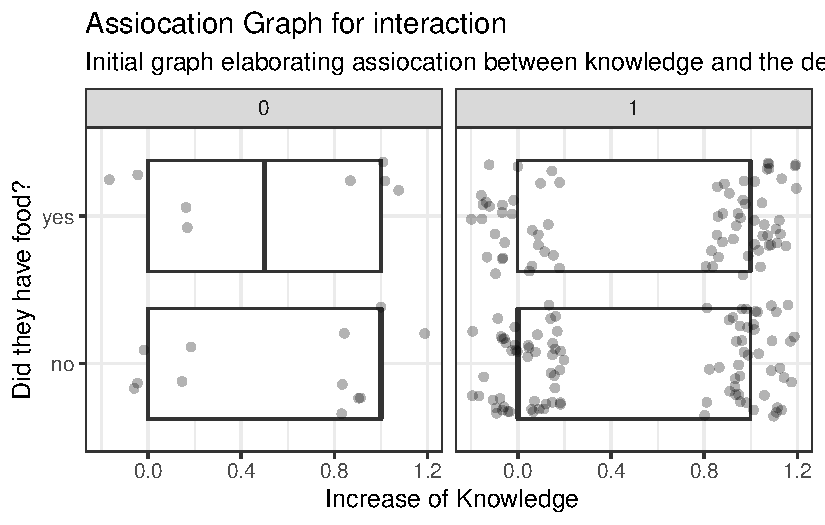
\includegraphics{Empircal-Research-final_files/figure-pdf/unnamed-chunk-2-1.pdf}

}

\end{figure}

\begin{Shaded}
\begin{Highlighting}[]
\NormalTok{int\_graph2 }\OtherTok{\textless{}{-}} \FunctionTok{gf\_boxplot}\NormalTok{(Food\_Ran\_Out }\SpecialCharTok{\textasciitilde{}}\NormalTok{ Increased\_Yield }\SpecialCharTok{|}\NormalTok{ Increased\_Knowledge ,  }\AttributeTok{data =}\NormalTok{ data1) }\SpecialCharTok{\%\textgreater{}\%}
  \FunctionTok{gf\_jitter}\NormalTok{(}\AttributeTok{alpha =} \FloatTok{0.3}\NormalTok{, }\AttributeTok{width =} \FloatTok{0.2}\NormalTok{) }\SpecialCharTok{\%\textgreater{}\%}
   \FunctionTok{gf\_labs}\NormalTok{(}\AttributeTok{subtitle =} \StringTok{"Initial graph elaborating assiocation between Yield and the decrease of no food"}\NormalTok{,}
          \AttributeTok{title =} \StringTok{"Assiocation Graph for interaction"}\NormalTok{,}
          \AttributeTok{x =} \StringTok{" Increase of Food yield"}\NormalTok{,}
          \AttributeTok{y =} \StringTok{"Did they have food?"}\NormalTok{, }
\NormalTok{           )}

\NormalTok{int\_graph2}
\end{Highlighting}
\end{Shaded}

\begin{figure}[H]

{\centering 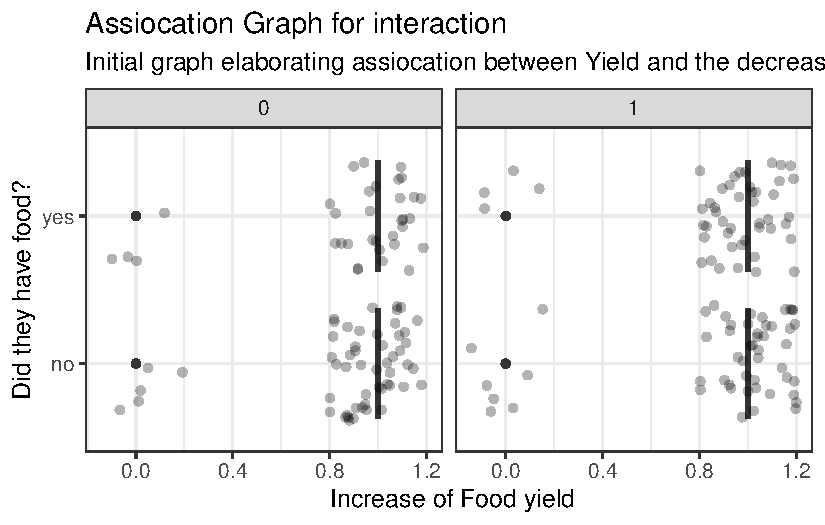
\includegraphics{Empircal-Research-final_files/figure-pdf/unnamed-chunk-3-1.pdf}

}

\end{figure}

\textbf{Returning to the question we have in mind :}

do the programs affect the individual's intellectuality and yield where
it makes sure that there is less food deprivation occurring more often.

ANSWER: Most definitely yes because we can observe an increase or a
difference in the amount of people who had food and did/didnt take the
program. I believe this makes my research question a topic worth going
into and evaluating. We could conclude hesitantly so far that the
programs have caused an increase in knowledge and indirectly influence
our yield which has caused a effect in the amount of food deprived
people.

\hypertarget{our-model}{%
\paragraph{Our Model}\label{our-model}}

\begin{Shaded}
\begin{Highlighting}[]
\NormalTok{model\_fitRan }\OtherTok{\textless{}{-}} \FunctionTok{glmmTMB}\NormalTok{(}\FunctionTok{factor}\NormalTok{(Food\_Ran\_Out) }\SpecialCharTok{\textasciitilde{}}\NormalTok{ Increased\_Knowledge}\SpecialCharTok{*}\NormalTok{Increased\_Yield }\SpecialCharTok{+}\NormalTok{ Age\_Group }\SpecialCharTok{+}\NormalTok{ Gender }\SpecialCharTok{+}
\NormalTok{                  (}\DecValTok{1}\SpecialCharTok{|}\NormalTok{Partner), }
                 \AttributeTok{data =}\NormalTok{ data1, }
                 \AttributeTok{family =} \FunctionTok{binomial}\NormalTok{(}\AttributeTok{link =} \StringTok{\textquotesingle{}logit\textquotesingle{}}\NormalTok{),}
                 \AttributeTok{na.action =} \StringTok{\textquotesingle{}na.fail\textquotesingle{}}\NormalTok{,}
                 \AttributeTok{REML =} \ConstantTok{FALSE}\NormalTok{)}


\FunctionTok{msummary}\NormalTok{(model\_fitRan)}
\end{Highlighting}
\end{Shaded}

\begin{verbatim}
 Family: binomial  ( logit )
Formula:          
factor(Food_Ran_Out) ~ Increased_Knowledge * Increased_Yield +  
    Age_Group + Gender + (1 | Partner)
Data: data1

     AIC      BIC   logLik deviance df.resid 
   256.5    282.4   -120.3    240.5      180 

Random effects:

Conditional model:
 Groups  Name        Variance Std.Dev.
 Partner (Intercept) 1.669    1.292   
Number of obs: 188, groups:  Partner, 10

Conditional model:
                                    Estimate Std. Error z value Pr(>|z|)  
(Intercept)                         -1.05722    1.04453  -1.012   0.3115  
Increased_Knowledge                  0.62317    1.16513   0.535   0.5928  
Increased_Yield                     -0.14140    0.77976  -0.181   0.8561  
Age_Group50_plus                    -0.83572    0.38542  -2.168   0.0301 *
Age_Groupunder_30                   -0.73642    0.44092  -1.670   0.0949 .
Gendermale                          -0.03445    0.33332  -0.103   0.9177  
Increased_Knowledge:Increased_Yield -0.25721    1.19300  -0.216   0.8293  
---
Signif. codes:  0 '***' 0.001 '**' 0.01 '*' 0.05 '.' 0.1 ' ' 1
\end{verbatim}

\textbf{summary of model:}

\begin{itemize}
\item
  \textbf{Model:} glmmTMB is form of regression which uses a
  mixed-effects linear model which is great for binomial regression. It
  is also used for random effects to which the parameter
  \texttt{Partner} would be our random effects.
\item
  \textbf{Interaction term:} we established an interaction predictor
  between \texttt{Increased\_Yield} * \texttt{Increased\_Knowledge} so
  that is elaborated in this model
\item
  \textbf{na.action and na.fail:} will fail the model if there are any
  missing data
\item
  \textbf{Reml:} is set to \textbf{\texttt{FALSE}}, which means that the
  model is fitted using maximum likelihood estimation, rather than
  restricted maximum likelihood estimation.

  \textbf{Results of model:}
\item
  \textbf{Rationale =} The logic for the predictors still remains the
  same. However, the Random effects I based it on The Partner because i
  believed it would be a bad traditional predictor because all the
  Organizations included have the same goal so theoretical it should be
  a bad predictor. It also fits the criteria we said in class that it
  must be a location, time, or identity which it is. I did not get any
  convergence problems so that's a good identification that it is a good
  RE effect. However, we have a high AIC and BIC relative to our
  observation so we should continue testing our model to see if there is
  correlation.
\item
  \textbf{SUMMARY EXPLANATION}

  Random effect variance estimate was overall good showing that the
  inclusion of partner is correct based on the STd. dev.

  \texttt{Partner\ (intercept)\ 1.669\ Variance\ 1.292\ std.\ Dev}

  \texttt{number\ of\ obs:\ 188,\ groups:\ Partner,\ 10}

  \hypertarget{assessments}{%
  \subsection{Assessments}\label{assessments}}

  \textbf{Dredge}

\begin{Shaded}
\begin{Highlighting}[]
\NormalTok{dredged }\OtherTok{\textless{}{-}} \FunctionTok{dredge}\NormalTok{(model\_fitRan, }\AttributeTok{rank =} \StringTok{\textquotesingle{}BIC\textquotesingle{}}\NormalTok{)}
\FunctionTok{head}\NormalTok{(dredged)}
\end{Highlighting}
\end{Shaded}

\begin{verbatim}
Global model call: glmmTMB(formula = factor(Food_Ran_Out) ~ Increased_Knowledge * 
    Increased_Yield + Age_Group + Gender + (1 | Partner), data = data1, 
    family = binomial(link = "logit"), na.action = "na.fail", 
    REML = FALSE, ziformula = ~0, dispformula = ~1)
---
Model selection table 
  cnd((Int)) dsp((Int)) cnd(Age_Grp) cnd(Gnd) cnd(Inc_Knw) cnd(Inc_Yld) df
1    -1.0270          +                                                  2
5    -1.3970          +                             0.4583               3
2    -0.7804          +            +                                     4
9    -0.8897          +                                         -0.1961  3
3    -1.0170          +                     +                            3
6    -1.0960          +            +                0.3799               5
    logLik   BIC delta weight
1 -124.076 258.6  0.00  0.690
5 -123.375 262.5  3.83  0.101
2 -120.838 262.6  4.00  0.094
9 -124.015 263.7  5.11  0.054
3 -124.071 263.9  5.23  0.051
6 -120.379 266.9  8.32  0.011
Models ranked by BIC(x) 
Random terms (all models): 
  cond(1 | Partner)
\end{verbatim}

  \textbf{Explanation:}
\item
  This indicates to us the inclusion of \texttt{(1\textbar{}Partner)}
  was a smart decision and we should proceed with our assessment!

  \textbf{Normality of Residuals}

\begin{Shaded}
\begin{Highlighting}[]
\FunctionTok{gf\_histogram}\NormalTok{(}\SpecialCharTok{\textasciitilde{}}\FunctionTok{resid}\NormalTok{(model\_fitRan), }\AttributeTok{data =}\NormalTok{ data1, }\AttributeTok{bins =} \DecValTok{6}\NormalTok{)}\SpecialCharTok{|\textgreater{}}
  \FunctionTok{gf\_labs}\NormalTok{(}\AttributeTok{title =} \StringTok{"Histogram: Normality of residuals"}\NormalTok{, }\AttributeTok{x =} \StringTok{"residuals"}\NormalTok{, }\AttributeTok{y =} \StringTok{"count"}\NormalTok{)}
\end{Highlighting}
\end{Shaded}

  \begin{figure}[H]

  {\centering 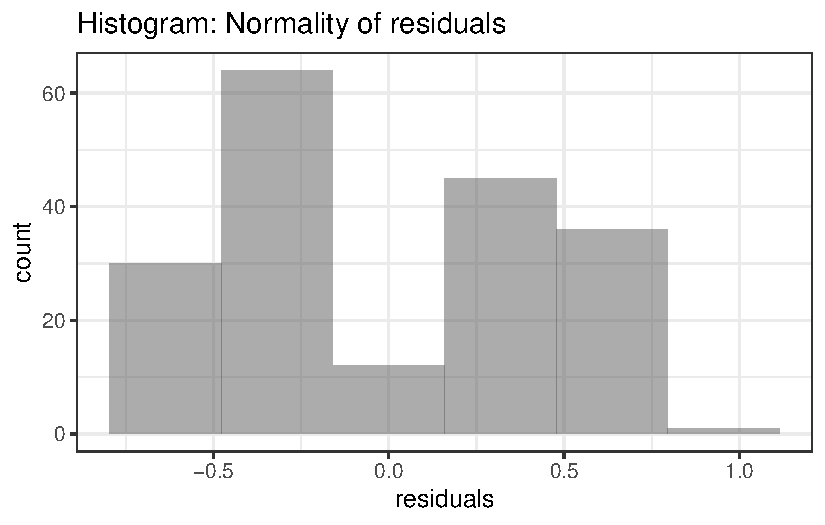
\includegraphics{Empircal-Research-final_files/figure-pdf/unnamed-chunk-6-1.pdf}

  }

  \end{figure}

  \textbf{Explanation:}
\item
  Normality of residuals refers to the assumption that the residuals of
  a statistical model are normally distributed. Residuals are the
  differences between the observed values and the predicted values from
  the model. If the residuals are normally distributed, it means that
  the model is capturing the underlying pattern in the data and that the
  model is a good fit for the data.

  A good indication of normality of residuals is when the histogram of
  residuals is approximately bell-shaped and symmetric. \textbf{=
  FAILED}

  \textbf{With random effects ACF TEST}

\begin{Shaded}
\begin{Highlighting}[]
\NormalTok{s245}\SpecialCharTok{::}\FunctionTok{gf\_acf}\NormalTok{(}\SpecialCharTok{\textasciitilde{}}\FunctionTok{resid}\NormalTok{(model\_fitRan))}\SpecialCharTok{|\textgreater{}}
\FunctionTok{gf\_lims}\NormalTok{(}\AttributeTok{y=}\FunctionTok{c}\NormalTok{(}\SpecialCharTok{{-}}\DecValTok{1}\NormalTok{,}\DecValTok{1}\NormalTok{))}\SpecialCharTok{|\textgreater{}}
   \FunctionTok{gf\_labs}\NormalTok{(}\AttributeTok{subtitle =} \StringTok{"Assement1"}\NormalTok{, }\AttributeTok{title =} \StringTok{"Independence Of Residuals"}\NormalTok{, )}
\end{Highlighting}
\end{Shaded}

  \begin{figure}[H]

  {\centering 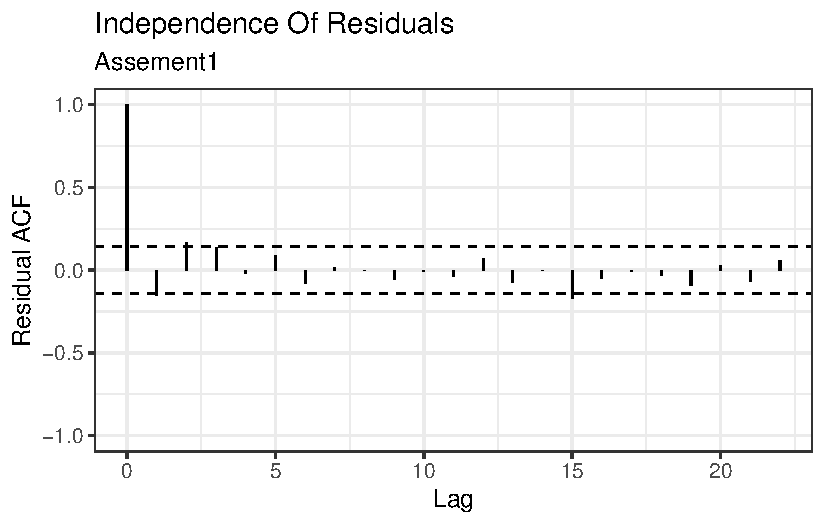
\includegraphics{Empircal-Research-final_files/figure-pdf/unnamed-chunk-7-1.pdf}

  }

  \end{figure}

  \textbf{Explanation:}
\item
  The \textbf{\texttt{gf\_acf}} function takes a time series object as
  input and creates a plot of the autocorrelation function (ACF) for the
  series. The ACF plot shows the correlation of a time series with its
  own lagged values. In other words, it shows how correlated a time
  series is with its own past values at different lags.

  The plot typically has the lag on the x-axis and the correlation
  coefficient on the y-axis. The plot also includes confidence bands to
  help identify statistically significant correlations.
\item
  Besides initial lag exceeding dashed areas, this assessment passes
  with good conditions

  \textbf{Scaled Residuals}

\begin{Shaded}
\begin{Highlighting}[]
\NormalTok{food\_sim }\OtherTok{\textless{}{-}} \FunctionTok{simulateResiduals}\NormalTok{(model\_fitRan)}
\FunctionTok{gf\_point}\NormalTok{(food\_sim}\SpecialCharTok{$}\NormalTok{scaledResiduals }\SpecialCharTok{\textasciitilde{}} \FunctionTok{fitted}\NormalTok{(model\_fitRan),}
\AttributeTok{alpha =} \FloatTok{0.2}\NormalTok{) }\SpecialCharTok{\%\textgreater{}\%}
\FunctionTok{gf\_labs}\NormalTok{(}
\AttributeTok{y =} \StringTok{\textquotesingle{}Scaled Residuals\textquotesingle{}}\NormalTok{)}
\end{Highlighting}
\end{Shaded}

  \begin{figure}[H]

  {\centering 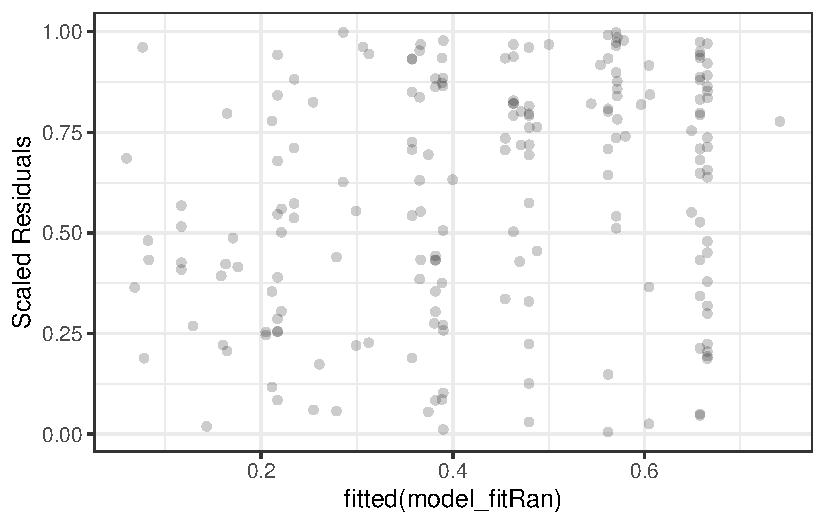
\includegraphics{Empircal-Research-final_files/figure-pdf/unnamed-chunk-8-1.pdf}

  }

  \end{figure}

  \textbf{Results:} Mean variance relationship looks great because we
  see a vertical relationship with minimal clustering in it.

  \textbf{Prediction Plot}

\begin{Shaded}
\begin{Highlighting}[]
\FunctionTok{ggpredict}\NormalTok{(model\_fitRan, }
          \FunctionTok{c}\NormalTok{(}\StringTok{"Increased\_Knowledge"}\NormalTok{, }\StringTok{"Increased\_Yield"}\NormalTok{), }
          \AttributeTok{type =} \StringTok{\textquotesingle{}re\textquotesingle{}}\NormalTok{) }\SpecialCharTok{|\textgreater{}} 
  \FunctionTok{plot}\NormalTok{() }
\end{Highlighting}
\end{Shaded}

  \begin{figure}[H]

  {\centering 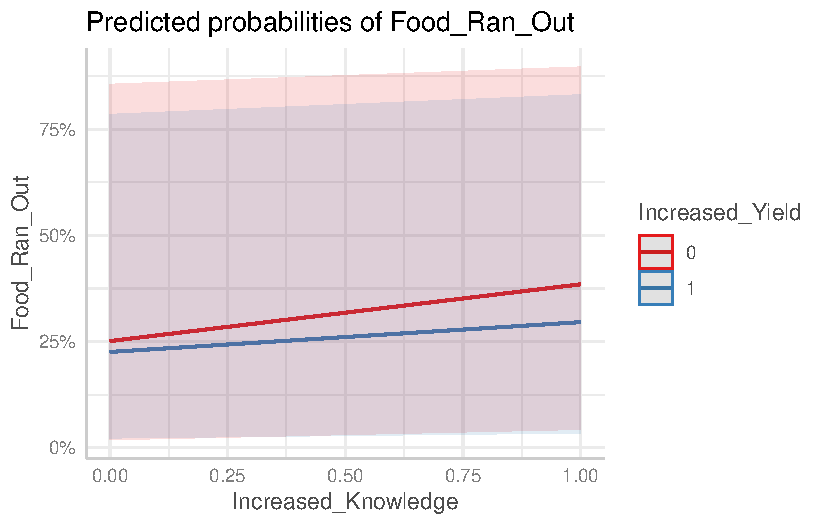
\includegraphics{Empircal-Research-final_files/figure-pdf/unnamed-chunk-9-1.pdf}

  }

  \end{figure}

  \textbf{Results:} I feel that this prediction plot demonstrates a
  better interaction than what we had in the previous test because it is
  showing us what we want to see in a interaction predictors. This is
  also a individual Average rather than population due to the dredge
  suggesting that a individual average is better.

  \hypertarget{conclusion}{%
  \subsection{Conclusion}\label{conclusion}}
\item
  \textbf{restated question:} do the programs affect the individual's
  intellectuality and yield where it makes sure that there is less food
  deprivation occurring more often. (is there a association between
  food\_ran\_out and increased\_knowledge/increased\_yield?)
\item
  \textbf{Answered based on previous test:} without random effects: can
  not be concluded from the results of the previous test to say that
  increased knowledge and increased yield resulted in less food
  deprivation if anything it could not be trusted for anything.
\item
  \textbf{Answered based on this test:} I can say more confidently that
  i can see that the interaction is giving us some insight that they
  might lead us to think that food deprivation occurs less. I would
  stick to these results because it gives a more affirmative result with
  appropriate measures followed. The prediction plot is completely
  different and is showing a interaction.

  \hypertarget{limitations-of-study}{%
  \subsection{Limitations of study}\label{limitations-of-study}}
\item
  \textbf{Time:} Being a junior with a double major, it was difficult to
  devote more time into this study because of other commitments.
\item
  \textbf{Knowledge:} I wish i knew more technical knowledge to do more
  assessments and an evaluations of the model I had!

  \hypertarget{implications-of-the-study}{%
  \subsection{Implications of the
  study}\label{implications-of-the-study}}
\item
  The extractions that we can make from this study are detrimental
  because it gives us justification to further expand our programs for
  food security. It is also necessary to establish initial steps to say
  that we can further expand or maintain these programs in the country
  because they are beneficial.

  \hypertarget{next-step}{%
  \subsection{Next step?}\label{next-step}}
\item
  deduce which variables are causing most influence on my response
  variable and make a concrete study on that independently.
\end{itemize}



\end{document}
